\documentclass[a4paper,11pt]{article}
\usepackage[encapsulated]{CJK}
\usepackage{ucs}
\usepackage[utf8x]{inputenc}
\usepackage{graphicx}       % front image
\usepackage{hyperref}       % links and email
\usepackage[english]{babel} % linebreaks for english words
\usepackage{eurosym}
\usepackage{pbox}           % linebreaks in tables

% footnotes in tables
\usepackage{footnote}
\makesavenoteenv{tabular}

% auto update years
\usepackage{datenumber}
\newcounter{dateone}
\newcounter{datetwo}
\newcommand{\difftoday}[3]{%
  \setmydatenumber{dateone}{\the\year}{\the\month}{\the\day}%
  \setmydatenumber{datetwo}{#1}{#2}{#3}%
  \addtocounter{datetwo}{-\thedateone}%
  \the\numexpr-\thedatetwo/365\relax
}

% opening
\title{Business plan\\YourCompanyLLC}
\author{YourName}

\begin{document}
\begin{CJK}{UTF8}{gbsn}
  \begin{titlepage}
    \centering
    \maketitle
    \thispagestyle{empty}   % discard page number
    
\includegraphics[width=2cm]{images/logo.png}
    \vfill
    {\raggedright
      YourName (CEO)\\
      YourAddress\\
      \href{mailto:yourmail@yourdomain.com}{yourmail@yourdomain.com}\\
    }
  \end{titlepage}

  \begin{abstract}
    Write here what it's all about.
  \end{abstract}

  \pagebreak
  \tableofcontents
  \pagebreak
  \section{SLE}
  我是中国人

  \section{Qualifications of founders}
  YourName has \difftoday{2010}{06}{01} years of experience in YourProfession.

  \section{MVP}

  \section{Strategy}
  % chart generated with Google chart API
  % http://chart.apis.google.com/chart?chs=300x300&chdl=A|B|C&chd=t:3,4,5&cht=p
  \begin{figure}[ht]
    \centering
    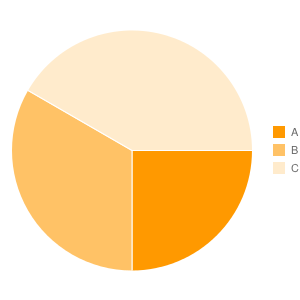
\includegraphics[width=5cm]{images/chart.png}
    \caption{A chart}
    \label{fig:chart}
  \end{figure}
  In Image \ref{fig:chart} you can see a chart.

  \section{Market and competition}
  Operating figures of competition:
  \begin{center}
    \begin{tabular}{l|l|r|r}
      Company & Product & Price (\$) & \pbox{20cm}{Sales\\(Mio. \$)}\\
      \hline
      A & 1 & 100 & 1000\\
      B\footnote{A footnote about B} & 2 & 100 & 1000\\
      C & 3 & 100 & 1000\\
    \end{tabular}
  \end{center}

  \section{Marketing}

  \section{Financial planning}

  \section{Equity requirements}

  \clearpage\end{CJK}
\end{document}

%%% Local Variables:
%%% mode: latex
%%% TeX-master: t
%%% End:
